\section{Experiment Details}
\label{supp:sec:experiment_details}

\subsection{DMLab Main Experiment}
Our DMLab main experiment is conducted on three levels with task IDs
\begin{itemize}
    \item{\texttt{explore\textunderscore{}goal\textunderscore{}locations\textunderscore{}large},}
    \item{\texttt{rooms\textunderscore{}watermaze},}
    \item{and \texttt{skymaze\textunderscore{}irreversible\textunderscore{}path\textunderscore{}hard}.}
\end{itemize}
We use no action repeats during training and evaluation.
For experiments with varying task difficulty, we select difficulty parameters ``room numbers'', ``spawn radius'', and ``built-in difficulty'' for these three levels, respectively.
We adopt environment wrappers and helper functions from \citet{petrenko2020sample} to flexibly and precisely maneuver task difficulties. 

Due to different task horizons, we tune the context length of Transformer-XL models and vary curricular trajectories accordingly. These differences are summarized in Table~\ref{supp:table:dmlab_main}.

\begin{table}[!htbp]
\caption{Experiment details on DMLab tasks. Columns ``Epoch'' denote the exact training epochs with best validation performance. We select these checkpoints for evaluation.
For task-difficulty-based curriculum, the column ``Training Trajectories'' with $n \times m$ entries means $n$ trajectories per difficulty level ($m$ levels in total). The column ``Sampled Episodes'' with $[i, j]$ entries means we first determine the number of episodes per difficulty level by uniformly sampling an integer from $[i, j]$ (inclusively).}
\centering
\vspace{0.1in}
\resizebox{1\textwidth}{!}{
\begin{tabular}{c|c|ccc|ccc}
\hline
\multirow{2}{*}{\textbf{\begin{tabular}[c]{@{}c@{}}Level\\ Name\end{tabular}}} & \multirow{2}{*}{\textbf{\begin{tabular}[c]{@{}c@{}}Context\\ Length\end{tabular}}} & \multicolumn{3}{c|}{\textbf{Task-Difficulty-Based Curriculum}}     & \multicolumn{3}{c}{\textbf{Learning-Progress-Based Curriculum}}    \\ \cline{3-8} 
                                                                               &                                                                                    & Epoch                   & Training Trajectories & Sampled Episodes & Epoch                   & Training Trajectories & Sampled Episodes \\ \hline
Goal Maze                                                                      & 500                                                                                & \multicolumn{1}{c|}{84} & 100 x 3               & {[}1, 5{]}       & \multicolumn{1}{c|}{88} & 300                   & 9                \\
Watermaze                                                                      & 400                                                                                & \multicolumn{1}{c|}{89} & 100 x 3               & {[}1, 5{]}       & \multicolumn{1}{c|}{80} & 300                   & 9                \\
Irreversible Path                                                              & 1600                                                                               & \multicolumn{1}{c|}{90} & 100 x 4               & {[}1, 3{]}       & \multicolumn{1}{c|}{97} & 400                   & 8                \\ \hline
\end{tabular}
}
\label{supp:table:dmlab_main}
\end{table}

RL oracles serve as source agents used to generate training data for our methods and the ``BC w/ Expert Data'' baseline.
They are trained with the PPO~\citep{schulman2017proximal} implementation from \citet{petrenko2020sample}.
The ``BC w/ Expert Data'' baselines have the same model architecture, training hyperparameters, and amount of training data as our method, but are trained solely on trajectories generated by the best performing RL oracles without cross-episodic attention.

\begin{table}[t!]
\caption{Evaluation results on DMLab, averaged over three tasks (Figure~\ref{fig:dmlab_core}).}
\label{supp:table:dmlab_main_avg_results}
\vspace{0.1in}
\centering
\resizebox{\textwidth}{!}{
\begin{tabular}{@{}cccccccccc@{}}
\toprule
\textbf{\begin{tabular}[c]{@{}c@{}}Ours (Task\\ Difficulty), Auto\end{tabular}} & \textbf{\begin{tabular}[c]{@{}c@{}}Ours (Task\\ Difficulty), Fixed\end{tabular}} & \textbf{\begin{tabular}[c]{@{}c@{}}Ours (Learning\\ Progress)\end{tabular}} & \textbf{\begin{tabular}[c]{@{}c@{}}DT (Mixed\\ Difficulty)\end{tabular}} & \textbf{\begin{tabular}[c]{@{}c@{}}DT (Single\\ Difficulty)\end{tabular}} & \textbf{\begin{tabular}[c]{@{}c@{}}AT (Mixed\\ Difficulty)\end{tabular}} & \textbf{\begin{tabular}[c]{@{}c@{}}AT (Single\\ Difficulty)\end{tabular}} & \textbf{\begin{tabular}[c]{@{}c@{}}BC w/ Expert\\ Data\end{tabular}} & \textbf{\begin{tabular}[c]{@{}c@{}}RL\\ (Oracle)\end{tabular}} & \textbf{\begin{tabular}[c]{@{}c@{}}Curriculum RL\\ (Oracle)\end{tabular}} \\ \midrule
51.4                                                                            & $\bestscore{54.4}$                                                                             & 32.4                                                                        & 35.3                                                                     & 11.7                                                                      & 42.7                                                                     & 33.4                                                                      & 14.2                                                                 & 40.6                                                           & 50.6                                                                      \\ \bottomrule
\end{tabular}
}
\end{table}


\subsection{DMLab Generalization}
\label{supp:sec:dmlab_generalization}
This series of experiments probe the zero-shot generalization capabilities of embodied agents in unseen maze configurations, out-of-distribution difficulty levels, and varying environment dynamics.
For the task ``Goal Maze w/ Unseen Mechanism'', we use the level with task ID \texttt{explore\textunderscore{}obstructed\textunderscore{}goals\textunderscore{}large}, which adds randomly opened and closed doors into the maze while ensuring a valid path to the goal always exists.
An example of an agent's ego-centric observation is visualized in Figure~\ref{supp:fig:obstructed_goal_maze}.

The task ``Irreversible Path (OOD. Difficulty)'' corresponds to configurations with the built-in difficulty of 1 (agents are only trained on difficulty up to 0.9, as noted in Table~\ref{table:dmlab_exp_setting}).
For tasks with varying environment dynamics, we directly test agents with an action repeat of 2. This is different from the training setting with no action repeat.

\begin{table}[t!]
\caption{Generalization results on DMLab, averaged over five settings (Figure~\ref{fig:dmlab_generalization}).}
\label{supp:table:dmlab_gen_avg_results}
\vspace{0.1in}
\centering
\resizebox{\textwidth}{!}{
\begin{tabular}{@{}ccccccccc@{}}
\toprule
\textbf{\begin{tabular}[c]{@{}c@{}}Ours (Task\\ Difficulty)\end{tabular}} & \textbf{\begin{tabular}[c]{@{}c@{}}Ours (Learning\\ Progress)\end{tabular}} & \textbf{\begin{tabular}[c]{@{}c@{}}DT (Mixed\\ Difficulty)\end{tabular}} & \textbf{\begin{tabular}[c]{@{}c@{}}DT (Single\\ Difficulty)\end{tabular}} & \textbf{\begin{tabular}[c]{@{}c@{}}AT (Mixed\\ Difficulty)\end{tabular}} & \textbf{\begin{tabular}[c]{@{}c@{}}AT (Single\\ Difficulty)\end{tabular}} & \textbf{\begin{tabular}[c]{@{}c@{}}BC w/ Expert\\ Data\end{tabular}} & \textbf{\begin{tabular}[c]{@{}c@{}}RL\\ (Oracle)\end{tabular}} & \textbf{\begin{tabular}[c]{@{}c@{}}Curriculum RL\\ (Oracle)\end{tabular}} \\ \midrule
$\bestscore{39.6}$                                                                      & 27.8                                                                        & 31.8                                                                     & 13.6                                                                      & 39.4                                                                     & 29.2                                                                      & 18.1                                                                 & 30.0                                                           & 37.6                                                                      \\ \bottomrule
\end{tabular}
}
\end{table}


\begin{figure}[ht]
    \centering
    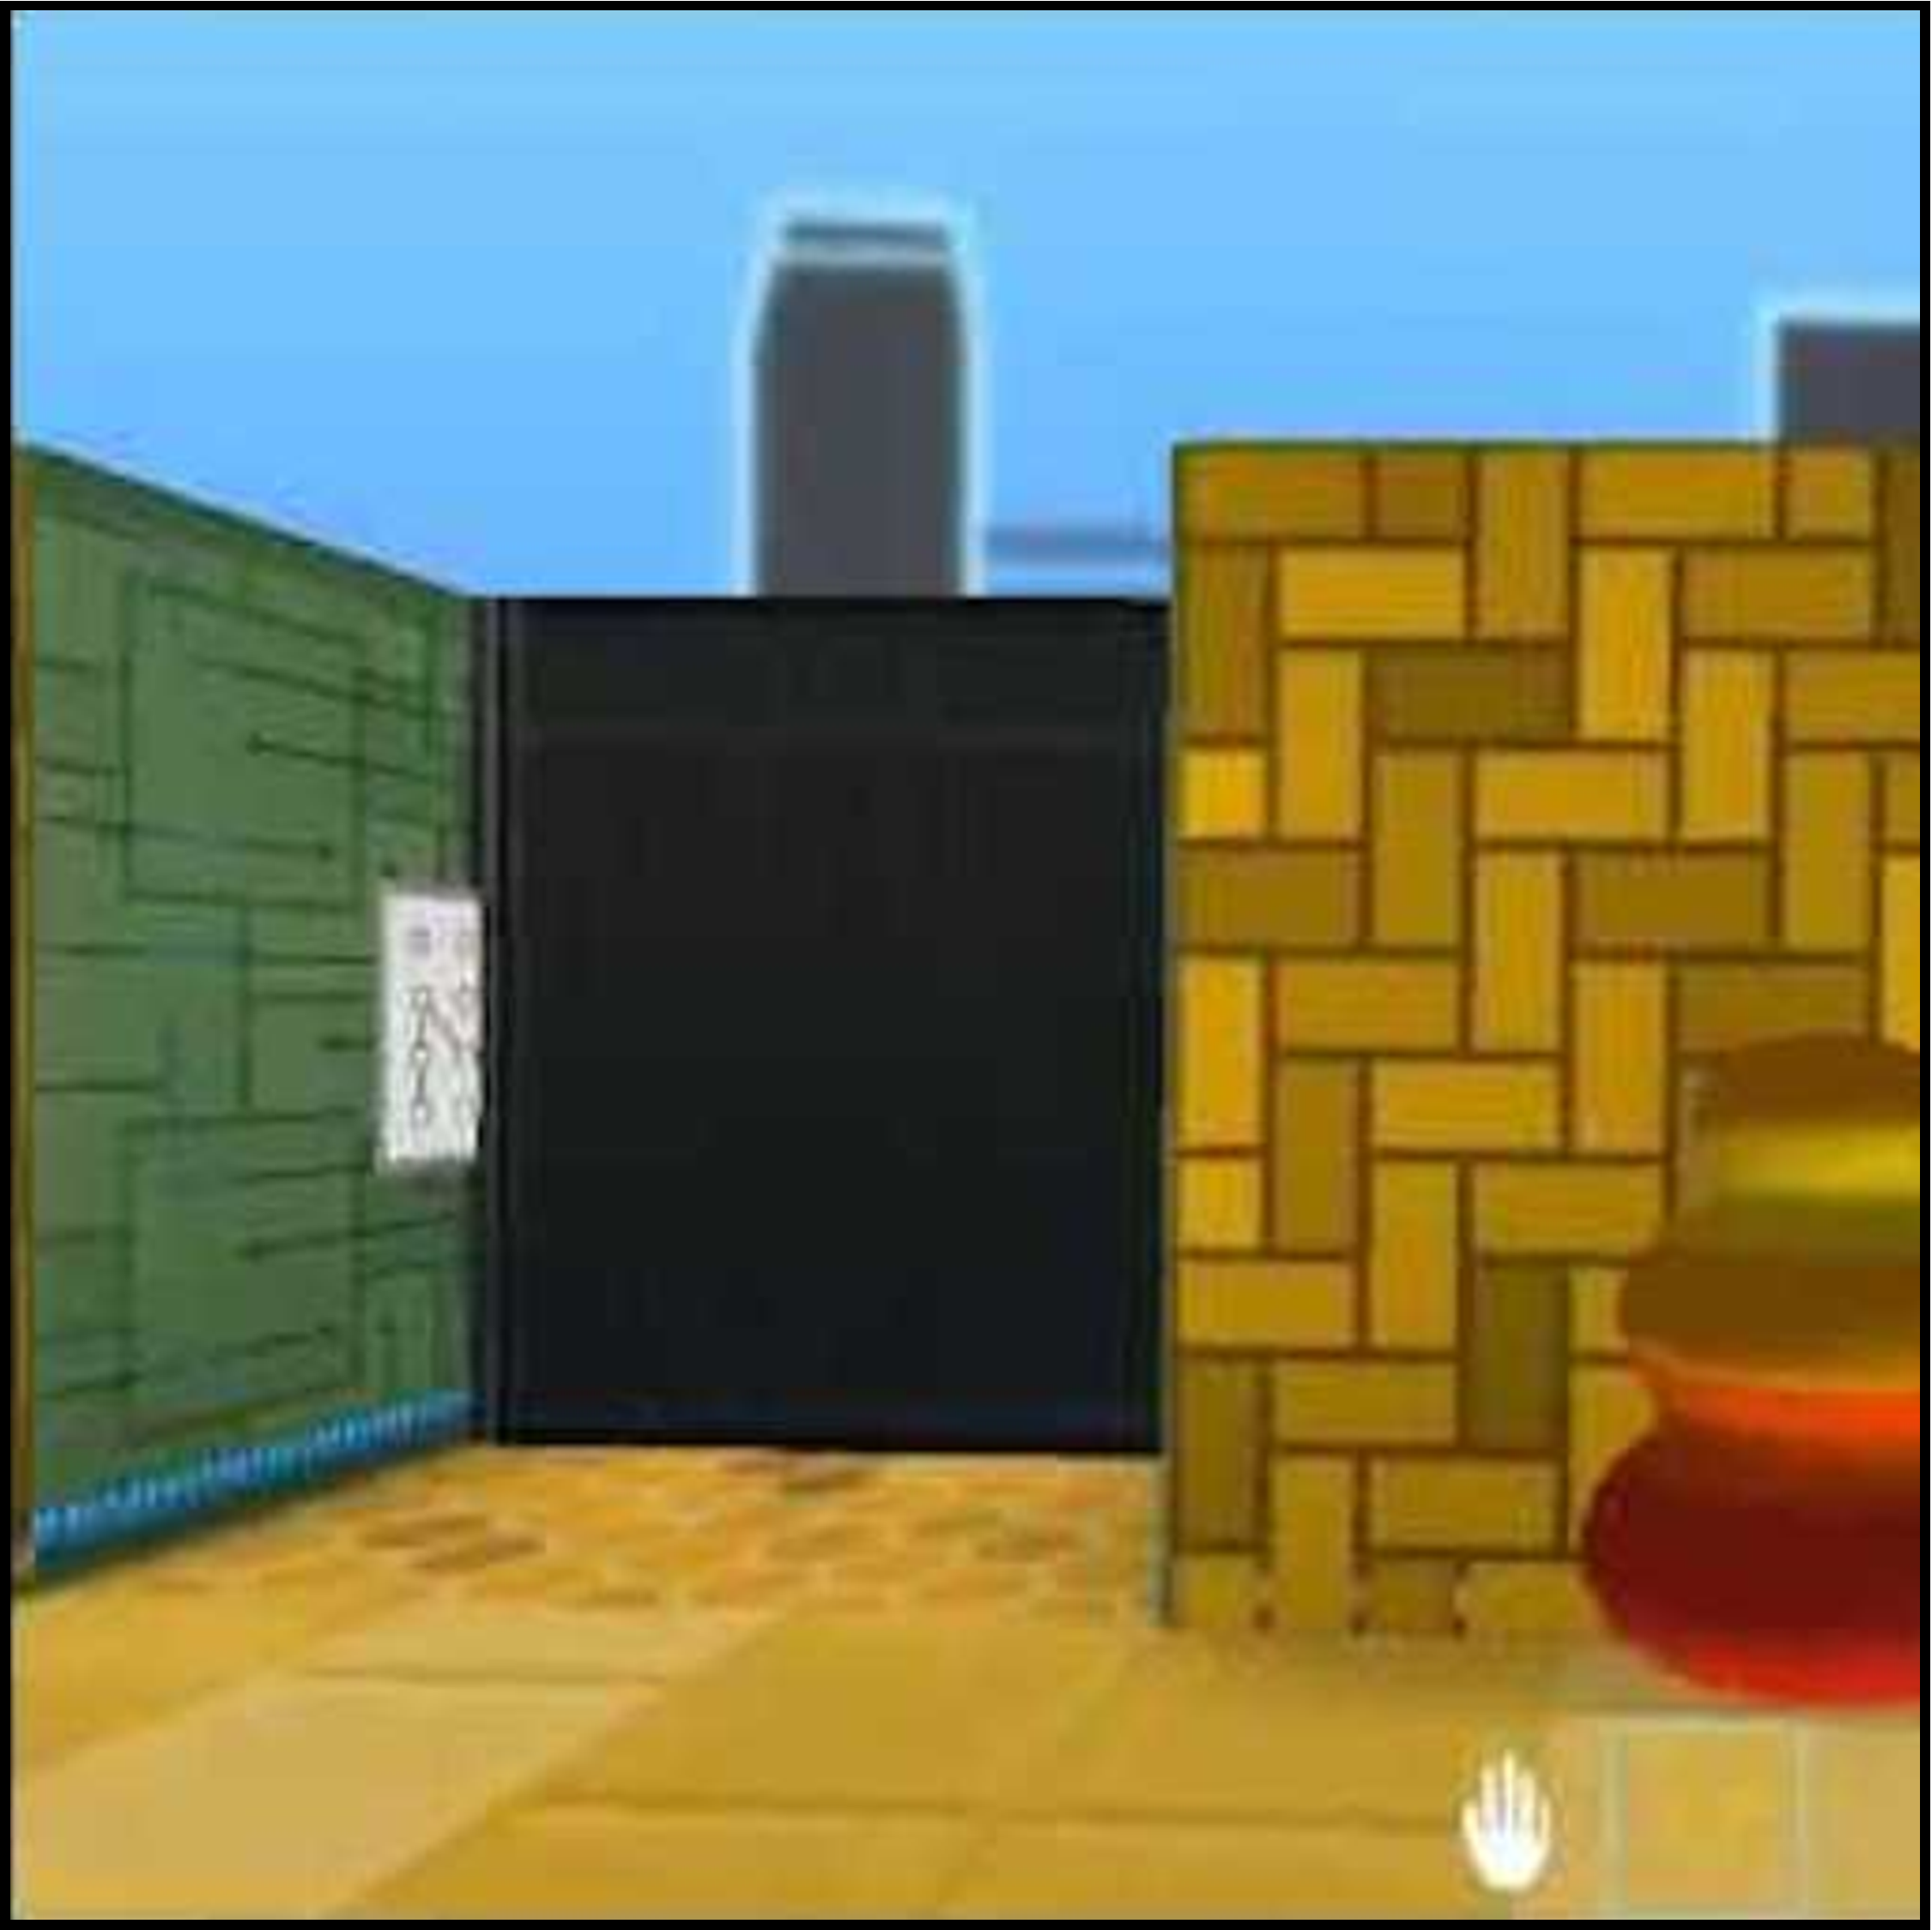
\includegraphics[scale=0.1]{appendix/figs/goal_maze_obstructed-fig.pdf}
    \caption{\textbf{A visualization of the task ``Goal Maze (Unseen Mechanism)''.} It includes doors that are randomly opened or closed.}
    \label{supp:fig:obstructed_goal_maze}
\end{figure}


\subsection{RoboMimic Main Experiment}
\label{supp:sec:robomimic_main}

We leverage the Multi-Human (MH) dataset from \citet{mandlekar2021matters}. It consists of demonstrations collected by operators with varying proficiency.
We construct the expertise-based curriculum by following the order of ``worse operators, okay operators, then better operators''.
We use a context length of 200 for both tasks. There are 90 trajectories per expertise level. To determine the number of trajectories per expertise level when constructing curricular data, we uniformly sample an integer from $[1, 5]$ (inclusively).
The ``Lift'' and ``Can'' tasks are solved after training for 33 epochs and 179 epochs, respectively.
We control for the same number of training epochs in subsequent ablation studies.

\subsection{Ablation Study on Curriculum Granularity}
\label{supp:sec:curriculum_granularity}

We perform this ablation with the task-difficulty-based curriculum on DMLab levels due to the ease of adjusting granularity.
The definition of varying levels of curriculum coarseness is listed in Table~\ref{supp:table:curriculum_granularity}.

\begin{table}[!htbp]
\caption{Definitions of varying levels of curriculum coarseness.}
\vspace{0.1in}
\centering
\begin{tabular}{@{}cccccc@{}}
\toprule
\textbf{Level Name} & \textbf{Difficulty Parameter} & \textbf{Test Difficulty} & \textbf{Fine} & \textbf{Medium} & \textbf{Coarse} \\ \midrule
Goal Maze           & Room Numbers                  & 20                       & 5→10→15       & 5→10            & 5→15            \\
Watermaze           & Spawn Radius                  & 580                      & 150→300→450   & 150→300         & 150→450         \\
Irreversible Path   & Built-In Difficulty           & 0.9                      & .1→.3→.5→.7   & .1→.5→.7        & .1→.3→.5        \\ \bottomrule
\end{tabular}
\label{supp:table:curriculum_granularity}
\end{table}


\subsection{Comparison of Curricula in RoboMimic}
\label{supp:sec:curriculum_comparison}

In IL settings, we further explored the efficacy of various curricula. For the RoboMimic tasks examined, we employed a learning-progress-based curriculum, ensuring the total training trajectories matched those of the expertise-based curriculum (i.e., 270 trajectories per task). All other parameters remained consistent, with the training data derived from RoboMimic's machine-generated dataset.

Table~\ref{supp:table:curriculum_comparison} indicates that when heterogeneous-quality human demonstrations are accessible, the expertise-based curriculum is preferable due to its superior performance over the learning-progress-based approach. Conversely, without expert demonstrations and relying solely on machine-generated data, the learning-progress-based curriculum is still commendable. It offers noteworthy results and surpasses offline RL methods like CQL~\citep{kumar2020conservative}, even though CQL is trained on the full RoboMimic dataset, encompassing 1500 trajectories for the Lift task and 3900 for the Can task.

\begin{table}[t!]
\caption{Results show the performance of different curricula on two robotic manipulation tasks: Lift and Can. Standard deviations are included.}
\label{supp:table:curriculum_comparison}
\vspace{0.1in}
\centering
\resizebox{\textwidth}{!}{
\begin{tabular}{@{}lccc@{}}
\toprule
\textbf{Task} & \textbf{Expertise-Based Curriculum} & \textbf{Learning-Progress-Based Curriculum} & \textbf{CQL}~\citep{kumar2020conservative} \\ \midrule
Lift          &  $100.0 \pm 0.0$      &    $32.0 \pm 17.0$                          & $2.7 \pm 0.9$ \\
Can           &  $100.0 \pm 0.0$       &    $30.0 \pm 2.8$                           & $0.0 \pm 0.0$ \\
Average       &  $\bestscore{100.0}$               &    $31.0$                                  & $1.4$         \\ \bottomrule
\end{tabular}
}
\end{table}
